\chapter {Simulation}

To do convex optimization, we choose the Python library CVXPY.
While a direct implementation of Algorithm [7] leads to extraordinarily large complexity, Candès and Romberg \cite {CaR05} showed that DS can be cast as a linear program, which we elaborate below.

\section {Method}

\subsection {Some notation}

Let us represent complex vectors and matrices by real vectors and matrices.
For \m {\V {x} \in \mathbb {C} ^{M}}, define the real representation \m {\mathcal {R} \SB {\V {x}}} of \m {\V {x}} to be
%
\DispNum {R:x:R2:M1} {
\mathcal {R} \SB {\V {x}}
\in &\mathbb {R} ^{2M} \notag \\
\mathcal {R} \SB {\V {x}} _{\SB {m}}
= &\begin {cases}
\mathfrak {Re} \SB {\V {x} _{\SB {m'}}}, & m =2m' \\
\mathfrak {Im} \SB {\V {x} _{\SB {m'}}}, & m =2m'+1 \\
\end {cases} \notag \\
m' 
= &0, 1, 2, \ldots, M-1 
}
%
The injection is obvious, and we may define \m {\mathcal {R} ^{-1}} so that
%
\DispNum {R:1:x::x:} {
\mathcal {R} ^{-1} \SB {\mathcal {R} \SB {\V {x}}}
=\V {x} 
}
%
Accordingly, the following generalization to complex matrices is valid, once we call the ring representation of complex numbers.
For \m {\M {A} \in \mathbb {C} ^{M_1 \D M_2}}, define real representation \m {\mathcal {R} \SB {\M {A}}} of \m {\M {A}} to be
%
\DispNum {R:A:R2:21} {
\mathcal {R} \SB {\M {A}}
\in &\mathbb {R} ^{2M_1 \D 2M_2} \notag \\
\mathcal {R} \SB {\M {A}} _{\SB {m_1,m_2}}
= &\begin {cases}
\mathfrak {Re} \SB {\M {A} _{\SB {m_1',m_2'}}}, & \RB {m_1, m_2} = \RB {2m_1', 2m_2'} \\
\mathfrak {Im} \SB {\M {A} _{\SB {m_1',m_2'}}}, & \RB {m_1, m_2} = \RB {2m_1'+1, 2m_2'} \\
-\mathfrak {Im} \SB {\M {A} _{\SB {m_1',m_2'}}}, & \RB {m_1, m_2} = \RB {2m_1', 2m_2'+1} \\
\mathfrak {Re} \SB {\M {A} _{\SB {m_1',m_2'}}}, & \RB {m_1, m_2} = \RB {2m_1'+1, 2m_2'+1} \\
\end {cases} \notag \\
m_1 
= &0, 1, 2, \ldots, M_1 -1 \notag \\
m_2 
= &0, 1, 2, \ldots, M_2 -1 
}

With these, we define

\DispNum {y:y:Ry:Ny} {
\tilde {\V {y}}
= &\mathcal {R} \SB {\V {y}}
\in \mathbb {R} ^{2 N_B ^2} \notag \\
%
\tilde {\V {g}}
= &\mathcal {R} \SB {\V {g}}
\in \mathbb {R} ^{2 N_{H,t} N_{H,r}} \notag \\
%
\tilde {\M {P}}
= &\mathcal {R} \SB {\M {P}}
\in \mathbb {R} ^{2 N_B ^2 \D 2 N_{H,t} N_{H,r}} \notag \\
%
\tilde {\M {P}} ^\Adj
= &\mathcal {R} \SB {\M {P} ^\Adj}
\in \mathbb {R} ^{2 N_B ^2 \D 2 N_{H,t} N_{H,r}} \notag \\
%
\tilde {\V {z}}
= &\mathcal {R} \SB {\V {z}}
\in \mathbb {R} ^{2 N_B ^2} 
}
%
so, by construction,
%
\Disp {
\V {\tilde {y}}
= \M {\tilde {P}} \V {\tilde {g}} +\V {\tilde {z}} 
}
%
And denote \m {\V {1}} to be the all-\m{1} vector, and \m {\V {0}} the all-\m{0} vector, whose dimension will be inferred from context.

\subsection {A Linear Program}

It is now straightforward to see that DS is equivalent to a linear program.

\Result
{Algorithm}
{
\begin {itemize}
\item Input \m {\M {P} \in \mathbb {C} ^{N_B^2 \D N_{H,t} N_{H,r}}}, \m {\V {y} \in \mathbb {C} ^{N_B^2}}, \m {\g_{\mathrm {DS}} > 0}.
%
\item Define \m {\tilde {\V {y}}, \tilde {\V {g}}, \tilde {\M {P}}, \tilde {\M {P}} ^\Adj, \tilde {\V {z}}}, according to \eqref {y:y:Ry:Ny}.
%
\item Compute the convex program
\DispNum {g:f:gf:S1} {
\hat {\tilde {\V {g}}}, \hat {\tilde {\V {f}}}
\leftarrow \begin {cases}
   \Min {\tilde {\V {g}}', \tilde {\V {f}}'}  & \IP {\V {1}, \tilde {\V {f}}'} \\
   \mathrm {subject} \; \mathrm {to} & \tilde {\V {g}}' \preceq \tilde {\V {f}}' \\
   & - \tilde {\V {g}}' \preceq \tilde {\V {f}}' \\
   & \tilde {\M {P}}^\dagger \tilde {\M {P}} \tilde {\V {g}}' \preceq \tilde {\M {P}}^\dagger \tilde {\V {y}} + \g_{\mathsf {DS}} \V {1} \\
   & - \tilde {\M {P}}^\dagger \tilde {\M {P}} \tilde {\V {g}}' \preceq - \tilde {\M {P}}^\dagger \tilde {\V {y}} + \g_{\mathsf {DS}} \V {1} \\
\end {cases} 
}
\item Convert
%
\DispNum {g:::R1:1g} {
\Hat{\V {g}}
\leftarrow \mathcal {R} ^{-1} \SB {\Hat{\T{\V {g}}}} 
}
\item Calculate
%
\DispNum {G:G:ve:1g} {
\hat {G}
\leftarrow \mathrm {vec}^{-1} \SB {\hat {g}} 
}
\item Calculate
%
\DispNum {H:H:KG:GK} {
\hat {\M {H}}
\leftarrow \M {K} \hat {\M {G}} \M {K}^\dagger 
}
\item Output \m {\hat {\M {H}}}.
\end {itemize}
}

\section {Variants}

We remark some possible variants of DS, either to enhance the accuracy, or to reduce the complexity, or both.

\subsection {Successive estimation of nonzero components}

We can apply DS more than once to better estimate the nonzero components;
let us call it the successive estimation \cite [CaT07].
We apply DS for the first time, and we extract largest components of the estimated vector.
Then we apply DS again, and we extract largest components of the second estimated vector.
Finally, we apply Moore–Penrose inverse to get the returned solution.
The resulting indices set has to be scrambled back according to the original indices.

\Result
{Algorithm}
{
\begin {itemize}
\item Let \m {\g_{\mathrm {DS}} \geq 0} be given, and \m {\M {P}}

\item Set
\Disp {
N_0
= &2 N_{H,t} N_{H,r}, \\
N_2
= &4 \lfloor \log N_{H,t} + \log N_{H,r} \rfloor, \\
N_1
= &\lfloor \R {N_0 N_2} \rfloor 
}

\item Apply DS to \m {\V {y}, \M {P}} to get \m {\hat {\V {g}}_0}, and call the \m {N_1} largest component of \m {\hat {\V {g}}_0} to be \m {\V {g}_1}, and corresponding columns of \m {\M {P}} to be \m {\M {P} _1}.

\item Apply DS to \m {\V {y}, \M {P}_1} to get \m {\hat {\V {g}}_1}, and call the \m {N_2} largest component of \m {\hat {\V {g}}_1} to be \m {\V {g}_2}, and corresponding columns of \m {\M {P}} to be \m {\M {P} _2}.

\item Apply Moore–Penrose inverse to \m {\V {y}, \M {P} _2} to get \m {\hat {\V {g}}_2}, which corresponds to \m {\hat {\V {g}}}.
\end {itemize}
}

If more than one stage of estimation is possible, that is, there are more than one dataset, the second stage may be run on the second dataset, and so on.
It is possible in theory to run it for three or more times.

From our observation, it is not conclusive whether the successive estimation method is more accurate, and whether a third or more stage is helpful.
It might have something to do with appropriately scaling \m {N_1, N_2} with respect to \m {N_{H,t}, N_{H,r}}.
We have not used this method in the plots included here.

\subsection {Basis pursuit denoising}

It is known that DS is equivalent to the basis pursuit denoising form below, for suitable \m {\l} (\cite {BoV04}, p.334).

\Disp {
\Hat {\V {g}}
\leftarrow \Min {\V {g}' \in \mathbb {C} ^{N_H^2}}
\RB {\VNm {\V {g}'} _1 + \l \VNm {\M {P}^\Adj \RB {\V {y} -\M {P} \V {g}'}} _\infty}
}

However, there is no simple way to determine the value of \m {\l} in advance.
We have tried basis pursuit denoising, with \m {\l = N_H^2 / \g_{\mathrm {DS}}} in the simulation.

\section {Result}

\subsection {Settings}

In addition to DS, we shall simulate OMP for three different stop conditions, Lasso, and Moore Penrose pseudoinverse (marked as LS which stands for least square).

To get some idea on the order of magnitude of noise-to-signal level, plug in some actual numbers.
Consider only path loss in the simplest form according to Friis Law.
Suppose the power of mobile phone antenna is \m {0.25} W,
the carrier frequency is \m {5} GHz,
the base station is \m {1.5} km away,
the noise is \m {–40} dB W.
If so, the noise-to-signal ratio is
\DispNum {1:8:02:24} {
10^{-4} \frac {1} {0.25} \R {\frac {5 \D 10^9 \D 4 \pi \D 1500} {3 \D 10^8}}
=0.224 
}

We use dimensionless noise level \m {\s} which takes value starting with \m {2^{-4}}, and being multiplied by powers of \m {2}, for \m {6} values.
We take \m {N_H} to be \m {6, 12, 18}, respectively.
For assorted plots, three series of plots are simulated.
The first series for \m {N_{H,t} = 2 N_B} and \m {N_{H,r} = 2 N_B}.
The second series for \m {N_{H,t} = 2 N_H} and \m {N_{H,r} = 3 N_H}.
The third series for \m {N_{H,t} = 3 N_H} and \m {N_{H,r} = 2 N_H}.
Unfortunately, this is very far from achieving the ideal values \eqref {N:B:4l:H2}, and this may be part of the reason the result is not as successful as expected.

Other parameters are fixed in these experiments.
The number of grid of quantization of phase shifters is \m {16}.
The number of paths \m {L = \R {N_{H,t} N_{H,r}}}.
The ratio of the wavelength of carrier over the antenna spacing, \m {\l _{\mathrm {ant}} / d _{\mathrm {ant}} = 1 / 2}.

Denote the threshold for DS to be \m {\g_{\mathrm {DS}}}, and similar threshold of Lasso to be \m {\g_{\mathrm {Lasso}}}.
We set \m {\g_{\mathrm {DS}} = \R {2 \log \RB {N_{H,t} N_{H,r}}}} as suggested in \cite {CaT07}.
For sake of comparison, \m {\g_{\mathrm {Lasso}} = \R {2 \log \RB {N_{H,t} N_{H,r}}}} too.
For OMP, we consult Cai and Wang \cite {CaW11} for \m {\ell _2}-norm condition in their Theorem 7, and \m {\ell _\infty}-norm condition in their Theorem 8.
We take \m {\h_{\mathrm {OMP}} = \R {2 \log \RB {N_{H,t} N_{H,r}}}} for \m {\infty}-norm condition, \m {\h_{\mathrm {OMP}} = \R {3 N_B}} for 2-norm condition.
The maximal number of iteration of CVXPY is set to be \m {32}, and that of OMP is set to be \m {4 N_B}.

Each data point for DS and Lasso is repeated for \m {256} times, and taken arithmetic average.
Other methods are repeated for more times: OMP for \m {4 \D 256} times, LS for \m {12 \D 256} times.

The parameters related to precision of the Newton step may be adjusted from CVXPY's class methods.
We set the maximum absolute tolerance to be \m {5 \D 10 ^ {-7}},
the maximum relative tolerance to be \m {5 \D 10 ^ {-6}},
the maximum feasible tolerance to be \m {5 \D 10 ^ {-7}}.
If the tolerance parameters are set too small, the program often gives overflowing values, perhaps because it was not able to find feasible solutions.
And if they are set too big, the Newton steps get imprecise and the performance is poorer.
It remains to determine the best choice of parameters.

For performance metric, we follow Lee, Gil, and Lee \cite [LGL16] to use
\DispNum {h:h:lo:vg} {
\tilde {\chi}
=\RB {
   \frac {\log_2 {\VNm {\V {h} -\hat {\V {h}}} _2}}
   {\log_2 {\VNm {\V {h}}_2}}
} _{\mathsf {avg}}, 
}
However, we remark that when \m {\VNm {\V {h}}_2} is small, this can blow up.
Indeed, since we did not consider a definite a channel model in this treatise, \m {\T {\chi}} may not necessarily be proportional to the channel capacity.

\subsection {Plots of \m {N_H = 6}}

In the following, we plot the reciprocal of noise level vs relative error norm in log scale, for different values and ratios of \m {N_H = 6} over \m {N_{B,t}} and \m {N_{B,r}}.

\begin {figure} [H]
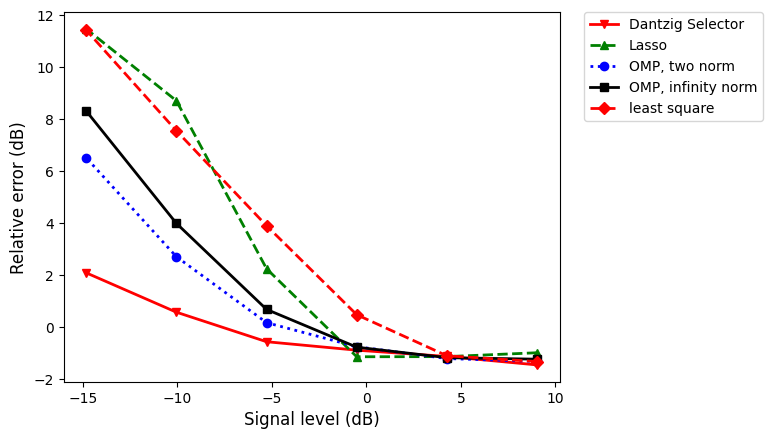
\includegraphics [width = \textwidth] {error-small-square-two.png}
\caption {\m {N_{B,t} = 3, N_{B,r} = 3, N_H = 6}, with \m {2} stages, error.}
\end {figure}

\begin {figure} [H]
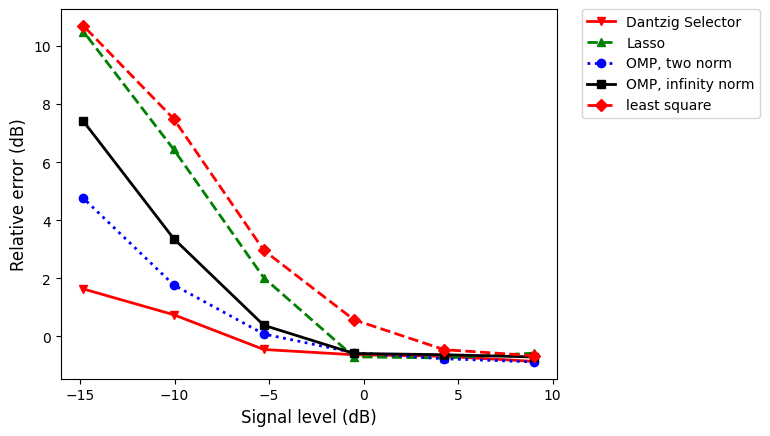
\includegraphics [width = \textwidth] {error-small-tall-two.png}
\caption {\m {N_{B,t} = 2, N_{B,r} = 3, N_H = 6}, with \m {2} stages, error.}
\end {figure}

\begin {figure} [H]
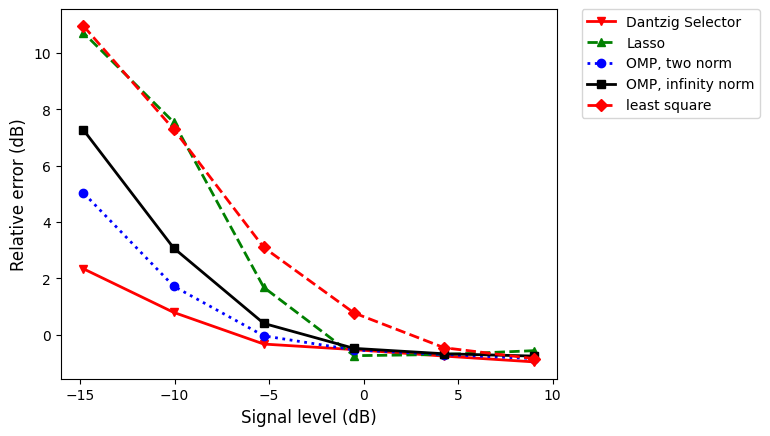
\includegraphics [width = \textwidth] {error-small-wide-two.png}
\caption {\m {N_{B,t} = 3, N_{B,r} = 2, N_H = 6}, with \m {2} stages, error.}
\end {figure}

\begin {figure} [H]
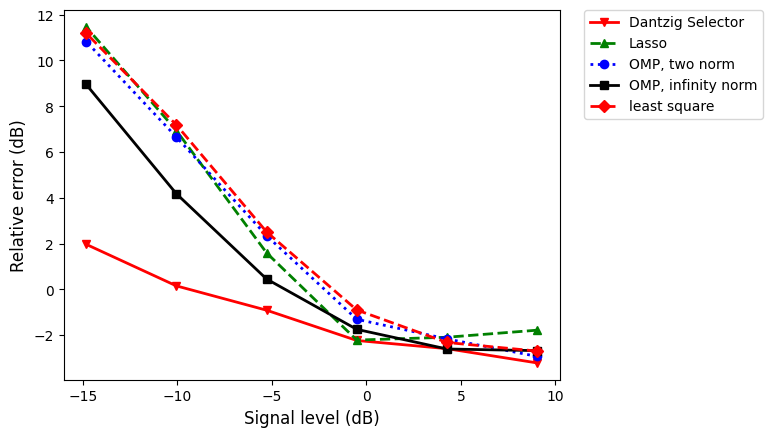
\includegraphics [width = \textwidth] {error-small-square-four.png}
\caption {\m {N_{B,t} = 3, N_{B,r} = 3, N_H = 6}, with \m {4} stages, error.}
\end {figure}

\begin {figure} [H]
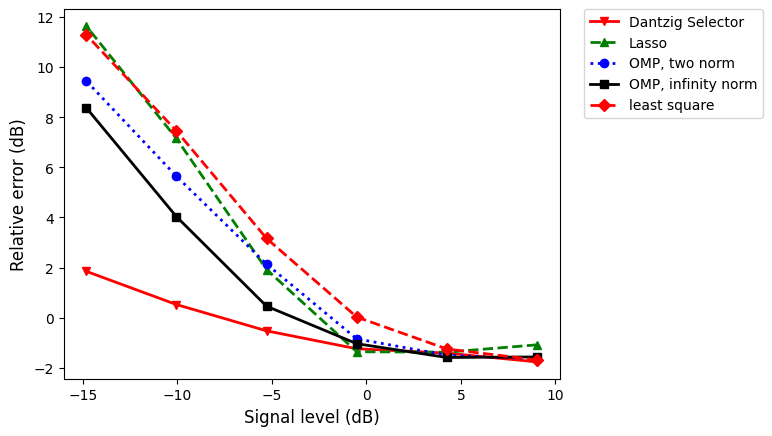
\includegraphics [width = \textwidth] {error-small-tall-four.png}
\caption {\m {N_{B,t} = 2, N_{B,r} = 3, N_H = 6}, with \m {4} stages, error.}
\end {figure}

\begin {figure} [H]
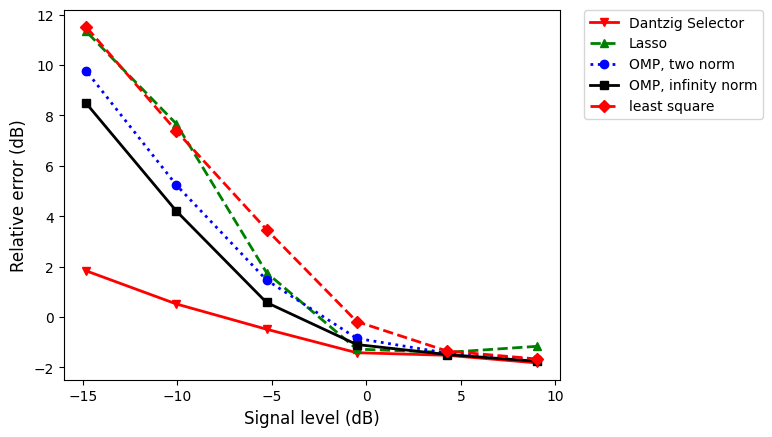
\includegraphics [width = \textwidth] {error-small-wide-four.png}
\caption {\m {N_{B,t} = 3, N_{B,r} = 2, N_H = 6}, with \m {4} stages, error.}
\end {figure}

\subsection {Plots of \m {N_H = 12}}

In the following, we plot the reciprocal of noise level vs relative error norm in log scale, for different values and ratios of \m {N_H = 12} over \m {N_{B,t}} and \m {N_{B,r}}.

\begin {figure} [H]
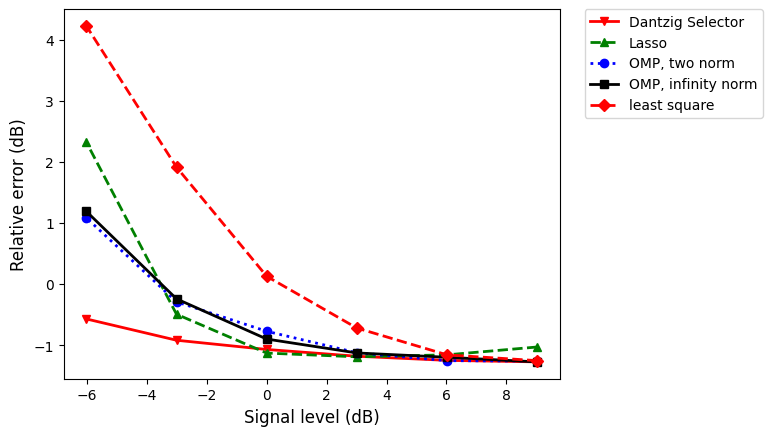
\includegraphics [width = \textwidth] {error-medium-square-two.png}
\caption {\m {N_{B,t} = 6, N_{B,r} = 6, N_H = 12}, with \m {2} stages, error.}
\end {figure}

\begin {figure} [H]
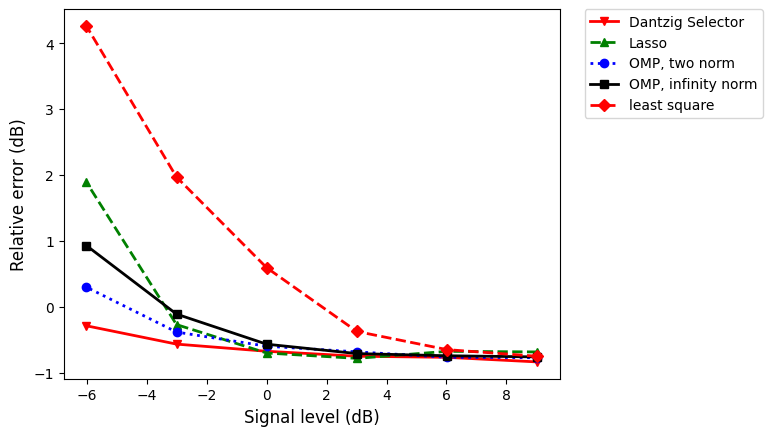
\includegraphics [width = \textwidth] {error-medium-tall-two.png}
\caption {\m {N_{B,t} = 4, N_{B,r} = 6, N_H = 12}, with \m {2} stages, error.}
\end {figure}

\begin {figure} [H]
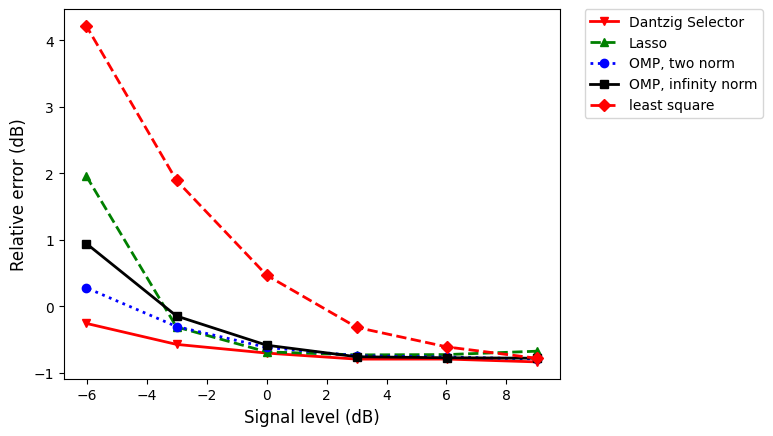
\includegraphics [width = \textwidth] {error-medium-wide-two.png}
\caption {\m {N_{B,t} = 6, N_{B,r} = 4, N_H = 12}, with \m {2} stages, error.}
\end {figure}

\begin {figure} [H]
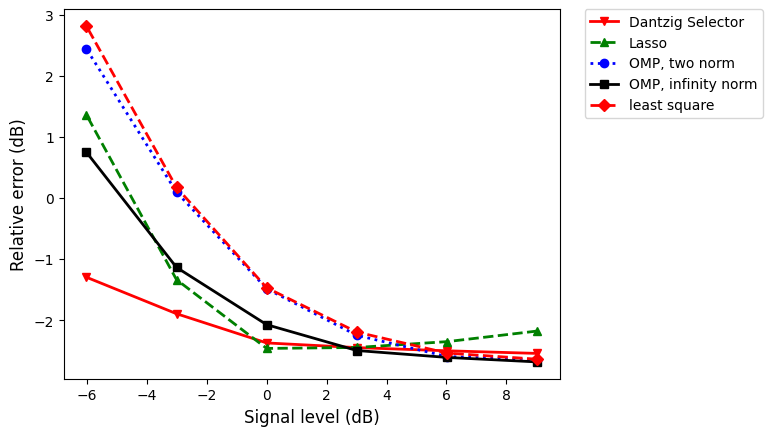
\includegraphics [width = \textwidth] {error-medium-square-four.png}
\caption {\m {N_{B,t} = 6, N_{B,r} = 6, N_H = 12}, with \m {4} stages, error.}
\end {figure}

\begin {figure} [H]
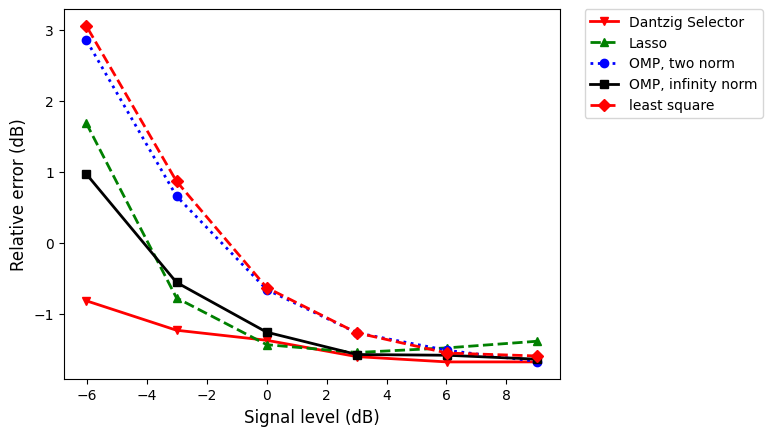
\includegraphics [width = \textwidth] {error-medium-tall-four.png}
\caption {\m {N_{B,t} = 4, N_{B,r} = 6, N_H = 12}, with \m {4} stages, error.}
\end {figure}

\begin {figure} [H]
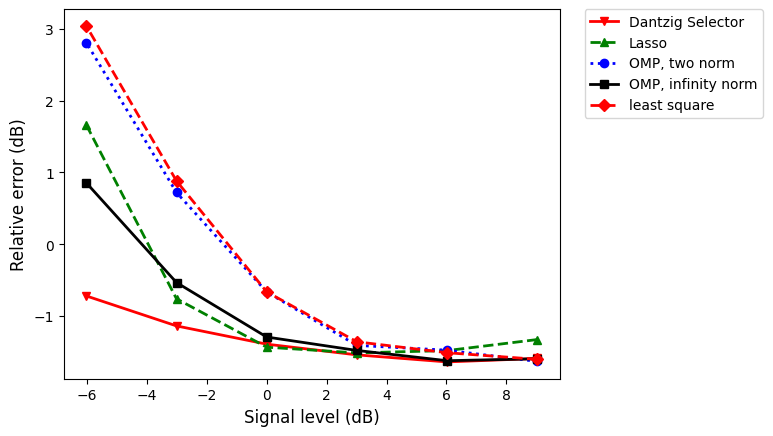
\includegraphics [width = \textwidth] {error-medium-wide-four.png}
\caption {\m {N_{B,t} = 6, N_{B,r} = 4, N_H = 12}, with \m {4} stages, error.}
\end {figure}


\subsection {Plots of \m {N_H = 18}}

In the following, we plot the reciprocal of noise level vs relative error norm in log scale, for different values and ratios of \m {N_H = 18} over \m {N_{B,t}} and \m {N_{B,r}}.

\begin {figure} [H]
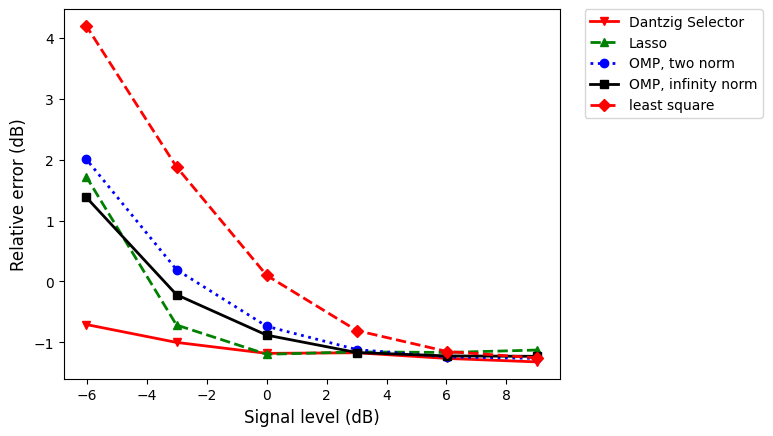
\includegraphics [width = \textwidth] {error-big-square-two.png}
\caption {\m {N_{B,t} = 12, N_{B,r} = 12, N_H = 18}, with \m {2} stages, error.}
\end {figure}

\begin {figure} [H]
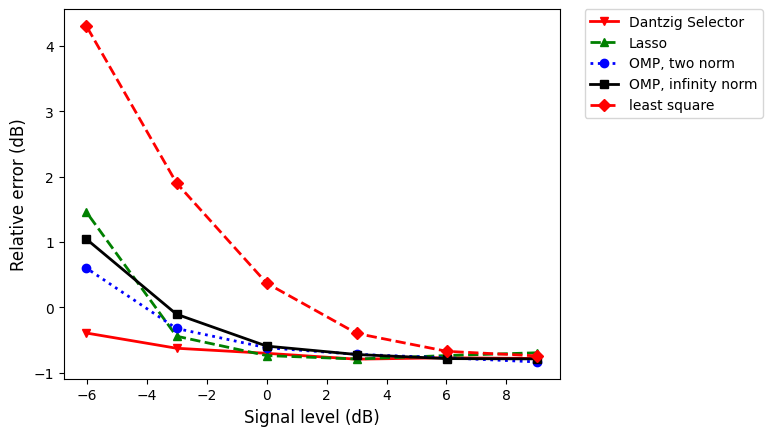
\includegraphics [width = \textwidth] {error-big-tall-two.png}
\caption {\m {N_{B,t} = 8, N_{B,r} = 12, N_H = 18}, with \m {2} stages, error.}
\end {figure}

\begin {figure} [H]
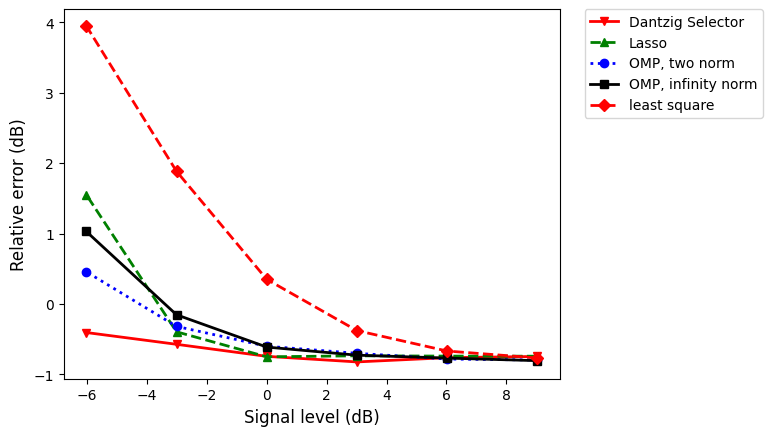
\includegraphics [width = \textwidth] {error-big-wide-two.png}
\caption {\m {N_{B,t} = 12, N_{B,r} = 8, N_H = 18}, with \m {2} stages, error.}
\end {figure}

\begin {figure} [H]
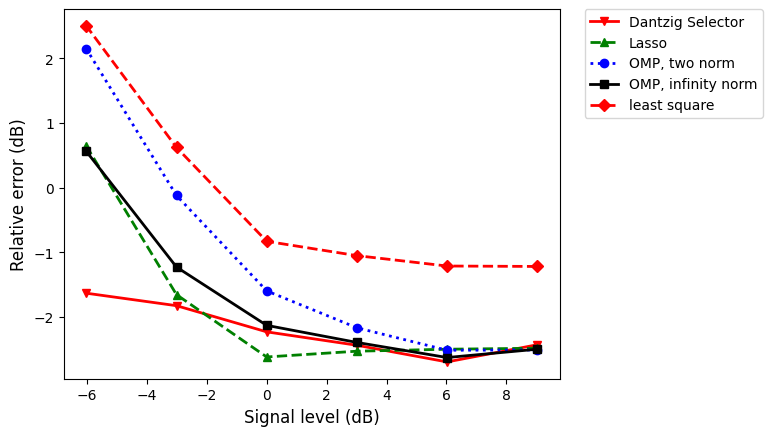
\includegraphics [width = \textwidth] {error-big-square-four.png}
\caption {\m {N_{B,t} = 12, N_{B,r} = 12, N_H = 18}, with \m {4} stages, error.}
\end {figure}

\begin {figure} [H]
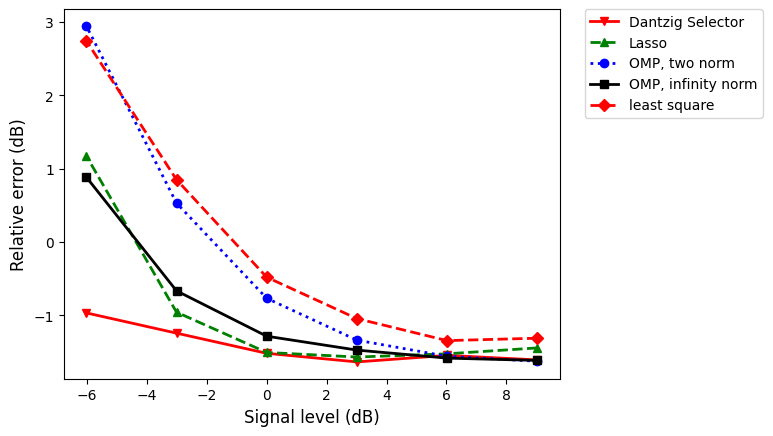
\includegraphics [width = \textwidth] {error-big-tall-four.png}
\caption {\m {N_{B,t} = 8, N_{B,r} = 12, N_H = 18}, with \m {4} stages, error.}
\end {figure}

\begin {figure} [H]
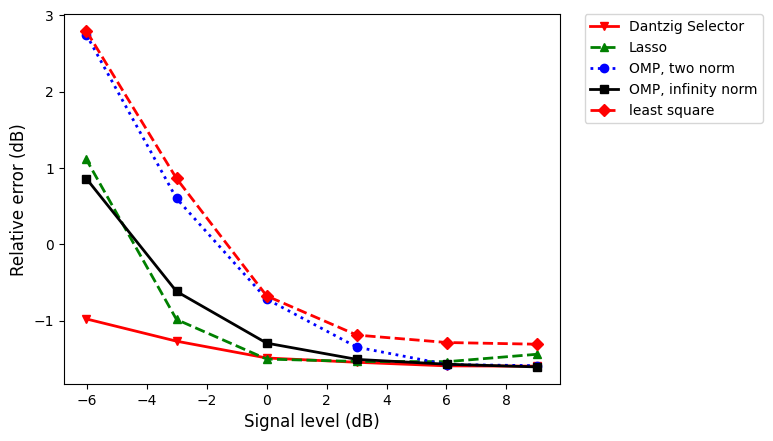
\includegraphics [width = \textwidth] {error-big-wide-four.png}
\caption {\m {N_{B,t} = 12, N_{B,r} = 8, N_H = 18}, with \m {4} stages, error.}
\end {figure}


\subsection {Plots of runtime}

Regarding runtime statistics, we only plot the case where \m {N_{B,t} = N_{B,r} = N_H /2} with \m {2} stages.

\begin {figure} [H]
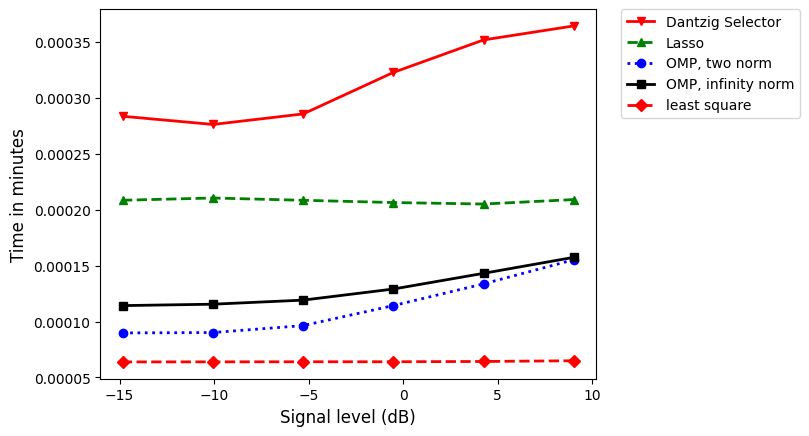
\includegraphics [width = \textwidth] {time-small-square-two.png}
\caption {\m {N_{B,t} = 3, N_{B,r} = 3, N_H = 6}, with \m {4} stages, time.}
\end {figure}


\begin {figure} [H]
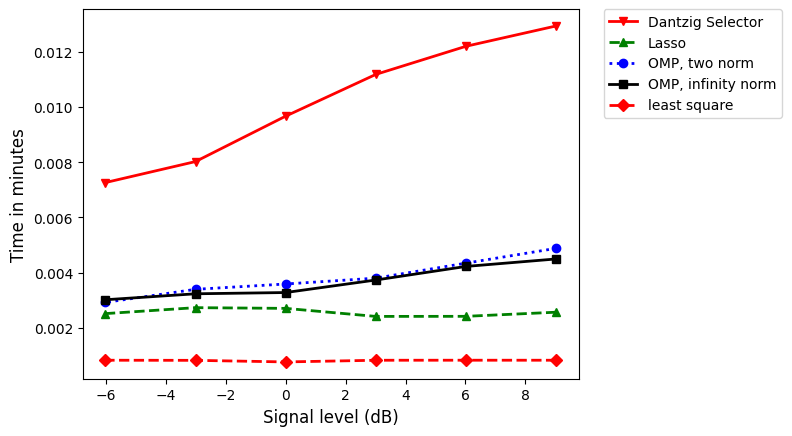
\includegraphics [width = \textwidth] {time-medium-square-two.png}
\caption {\m {N_{B,t} = 6, N_{B,r} = 6, N_H = 12}, with \m {4} stages, time.}
\end {figure}


\begin {figure} [H]
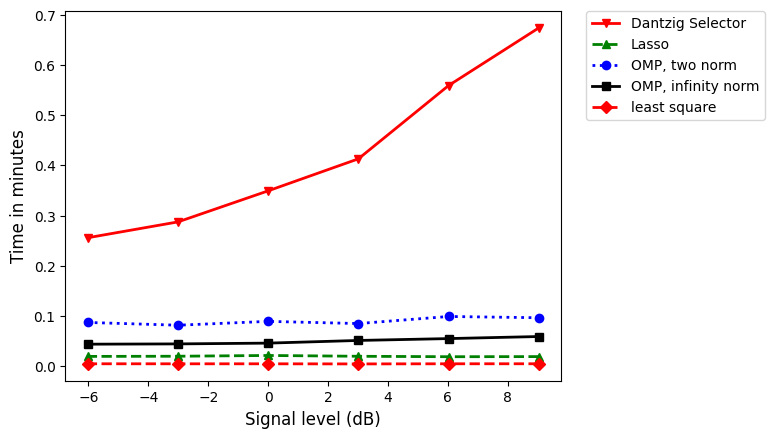
\includegraphics [width = \textwidth] {time-big-square-two.png}
\caption {\m {N_{B,t} = 9, N_{B,r} = 9, N_H = 18}, with \m {4} stages, time.}
\end {figure}


\subsection {Discussion}

From the simulation, DS outperforms other methods in most of the datasets.
With low noise, \m {\tilde {\chi} _{\mathrm {DS}} \approx \tilde {\chi} _{\mathrm {OMP}} \approx \tilde {\chi} _{\mathrm {Lasso}} \approx \tilde {\chi} _{\mathrm {LS}}}.
But with high noise, \m {\tilde {\chi} _{\mathrm {OMP}}, \tilde {\chi} _{\mathrm {Lasso}}, \tilde {\chi} _{\mathrm {LS}}} blow up quickly,
and it is usually true that \m {\tilde {\chi} _{\mathrm {DS}} \leq \tilde {\chi} _{\mathrm {OMP}} \leq \tilde {\chi} _{\mathrm {Lasso}} \leq \tilde {\chi} _{\mathrm {LS}}}.

For OMP, in Lee, Gil, and Lee \cite [LGL16], a high-complexity nonconvex program is used to design the sensing matrix, while we have here a low-complexity, random generation of beamforming matrices.
We keep in mind that a different design of sensing matrix, or a distribution of angles, will affect the performance of OMP.

For Lasso, \m {\g} (or \m {\l}) is also crucial to the performance, but cannot be obtained in advance.
Thus, for sake of comparison, we set the same threshold for Lasso and DS.
Still, there may be other values of \m {\g} (or \m {\l}) for which DS and Lasso are both better.

For DS itself, first, \m {\tilde {\chi} _{\mathrm {DS}}} certainly decreases as \m {\s} increases, but it does not decrease indefinitely.
Second, \m {\tilde {\chi} _{\mathrm {DS}}} decreases as \m {N_H} increases.
Third, when \m {N_{B,t} /N_{B,r}} is smaller, \m {\tilde {\chi} _{\mathrm {DS}}} is also smaller, because we have a higher sample rate.

Unfortunately, we report that CVXPY sometimes gives overflowing values, some of them as large as \m {10^{11}}.
This probably indicates some typical-looking output may in fact be unreliable.
Therefore we have discarded outputs larger than a given threshold, for instance \m {10^4}, and simply return the answer to be a Moore–Penrose inverse.

\m {\chi} is not shown in the figure, because the big O bound is much larger than \m {\tilde {\chi}}.
It is possible that the nonsparsity of \m {\V {g}} undermines the analysis in chapter 3, despite our attempts to account for that effect.
It is curious to see whether for very large \m {N_H}, whether \m {\tilde {\chi}} and \m {\tilde {\chi}} will be asymptotically close.

In figures 24 and 25, we reproduce two cases of success and failure of DS.
In both figures the true values of \m {\M {H}} entries are ordered by magnitude, and corresponding estimated values in the first and second stage are plotted against them.
When DS fails, the soft thresholding did not rule out smaller entries, thus a second application of DS on the wrong index set failed too.
When DS succeeded, the soft thresholding gave a reasonable guess of the nonzero components, thus a second application of DS on this index set refined the estimated values.


\bigskip
\begin {figure} [H]
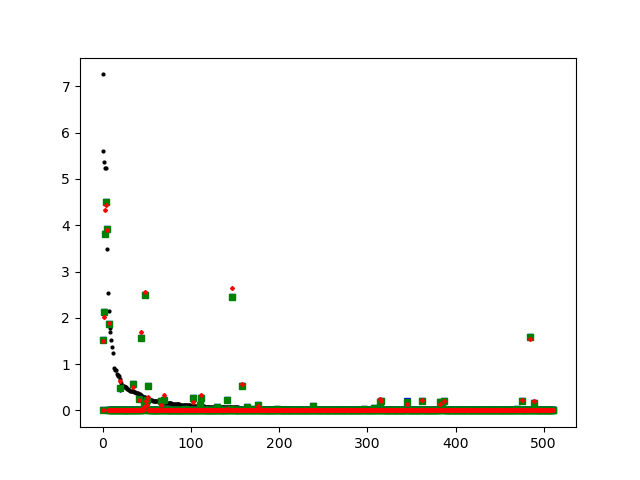
\includegraphics [width = 0.8 \textwidth] {scatter-ddss-failure.png}
\caption {A scatter plot of position versus magnitude for a case in which DS failed.}
\end {figure}
%
\begin {figure} [H]
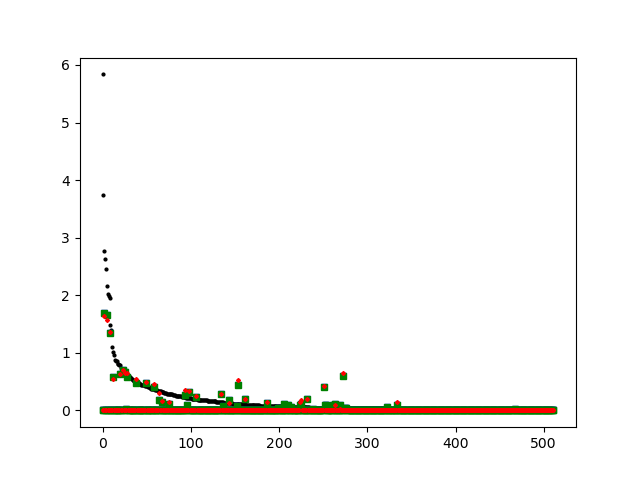
\includegraphics [width = 0.8 \textwidth] {scatter-ddss-success.png}
\caption {A scatter plot of position versus magnitude for a case in which DS succeeded.}
\end {figure}
\bigskip

\section {Complexity}

We discuss the complexity of DS, Lasso, and OMP.

\subsection {Dantzig Selector}

Suppose a linear program has an \m {N} dimensional variable and \m {M} inequality constraints, then its complexity is \m {\mathcal {O} \SB {N^2 M}}, assuming the Dantzig simplex method is used (\cite {BoV04}, p.6).
For our case, that would be \m {\mathcal {O} \SB {4 N_H ^4 \D 8 N_H^2} = \mathcal {O} \SB {N_H^6}}.
But other algorithms exist, where, in general, complexity of convex programs is difficult to analyze, as it is not easily to determine how many steps were calculated.

Alternatively, suppose Newton method is used.
Here, we have self-concordance for linear program.
Let \m {\V {g} _0} denote the starting value of \m {\V {g}'}, and \m {\V {g} ^{\star}} the the point of convergence.
Then the number of Newton steps is bounded \cite {BoV04} by
%
\Disp {
C_{\mathrm {Newton}}
= \RB {C_0 \VNm {\V {g}_0 -\V {g} ^{\star}}_1
+ \log_2 \log_2 \frac {1} {\e}}
}
%
If we just take that as the complexity bound for DS,
%
\DispNum {C:S:C0:1e'} {
C_{\mathrm {DS}}
= \RB {C_0 \VNm {\V {g}_0 -\V {g} ^{\star}}_1
+ \log_2 \log_2 \frac {1} {\e}} C_{\mathrm {step}}
}
%
Here \m {C_0} is constant related to implementation of Newton method, and \m {\e} the tolerance of error, and \m {C_{\mathrm {step}}} is the complexity of Newton step.

Every Newton step involves a inversion of \m {\mathcal {O} \SB {\M {P} ^\dagger \M {P}}}, having the same order of magnitude to the time needed for matrix multiplication.
Since the dimension of \m {\M {P} ^\dagger \M {P}} is \m {N_H^2}, the cost of inversion may be roughly considered to be \m {\mathcal {O} \SB {N_H^4}}, as we know from newer results on the complexity of matrix inversion.
That is, we suppose \m {C_{\mathrm {step}} = N_H^4}.

We take some liberty to assume that, at the start the iteration, the Moore–Penrose inverse was taken to be the initial value of \m {\V {g}_0}, namely
%
\DispNum {g:0:gL:Py} {
\V {g}_0
=\V {g}_{\mathrm {LS}}
= \RB {\M {P} ^\dagger \M {P}} ^{-1} \M {P} ^\dagger \V {y} 
}
%
By above, we may write the complexity of DS to be
%
\DispNum {C:S:Og:g1} {
C_{\mathrm {DS}}
=\mathcal {O} \SB {\VNm {\V {g}_{\mathrm {LS}} -\V {g} ^\star} _1} N_H^4 
}
%
Also assume
%
\DispNum {g:g:g;:;g} {
\V {g} ^\star
\approx \V {g} 
}
%
Indeed, this is the main thesis of our investigation.
And by restricted isometry, \m {\M {P}} has unity-normed, almost orthogonal columns, so
%
\DispNum {P:P:IN:H2} {
\M {P} ^\dagger \M {P}
\approx I _{N_{H}^2} 
}
%
Thus, by \eqref {g:0:gL:Py}, \eqref {C:S:Og:g1}, and \eqref {g:g:g;:;g},
%
\DispNum {C:S:Og:z1} {
C_{\mathrm {DS}}
=\mathcal {O} \SB {
   \VNm {\V {g} +\RB {\M {P} ^\dagger \M {P}} ^{-1} \M {P} ^\dagger \V {z}
   -\V {g}} _1} N_H^4
=\mathcal {O} \SB {\VNm {\M {P} ^\dagger \V {z}} _1} N_H^4 
}

We see that \m {\RB {\M {P} ^\dagger \V {z}} _{\SB {j}}} observes complex standard normal distribution.
If we agree that, for high probability,
%
\DispNum {O:j:sO:O1} {
\mathcal {O} \SB {\VNm {\M {P} ^\dagger \V {z}}}
= \s N_H^2 \mathcal {O} \RB {1} 
}
Then we simply have
%
\DispNum {C:S:ON:H6} {
C_{\mathrm {DS}}
=\mathcal {O} \SB {N_{H}^6} 
}

\subsection {Orthogonal matching pursuit}

Tropp and Gilbert \cite {TrG07a} discussed the complexity of OMP in the companion paper \cite {TrG07b}, giving
%
\DispNum {C:P:ON:NY} {
C_{\mathrm {OMP}}
=\mathcal {O} \SB {N_H^2 \log \RB {N_{B,r} N_{B,t}}}
}
%
Here \m {\log \RB {N_{B,r} N_{B,t}}} is small in our experiments, and if we dropped it, we may take
\DispNum {C:P:ON:H2} {
C_{\mathrm {OMP}}
=\mathcal {O} \SB {N_H^2}
}

\subsection {Lasso}

Lasso is equivalent to a quadratically constrained quadratic program, and there is not always a closed form for its complexity.
However, Lasso and DS are equivalent in certain conditions \cite {AsR10}, and we may suppose here they have the same complexity, \m {\mathcal {O} \SB {N_H^6}}.

Alternatively, an argument similar to the above one for DS is valid for Lasso.

Therefore we take
\DispNum {C:o:ON:H6} {
C_{\mathrm {Lasso}}
=\mathcal {O} \SB {N_H^6}
}

\subsection {Runtime statistics}

All plots included in this treatise, in total, took about one month to run.
Figures for \m {N_H = 18} each took about \m {3} days.
The computer has \m {32} GB RAM, and Intel Core i9 processor.
Simulation was run on Linux subsystem 2 of Windows 10.

Use \m {t_{\mathrm {OMP}} \SB {N_H}}, \m {t_{\mathrm {Lasso}} \SB {N_H}}, \m {t_{\mathrm {DS}} \SB {N_H}} to denote their respective time taken.
We here copy the arithmetic average (including different \m {\s}) of simulated values below, in seconds.
They are:
\m {t_{\mathrm {OMP}} \SB {12}  = 0.0119,}
\m {t_{\mathrm {OMP}} \SB {16} = 0.0297, }
\m {t_{\mathrm {OMP}} \SB {20}  = 0.0600,}
\m {t_{\mathrm {OMP}} \SB {24} = 0.155, }
%
\m { t_{\mathrm {Lasso}} \SB {12}  = 0.0436,}
\m { t_{\mathrm {Lasso}} \SB {16} = 0.176, }
\m { t_{\mathrm {Lasso}} \SB {20}  = 0.471,}
\m { t_{\mathrm {Lasso}} \SB {24} = 1.26, }
%
\m { t_{\mathrm {DS}} \SB {12}  = 0.357,}
\m { t_{\mathrm {DS}} \SB {16} = 2.07, }
\m { t_{\mathrm {DS}} \SB {20}  = 29.8,}
\m { t_{\mathrm {DS}} \SB {24} = 91.5}

Simulation illustrates that \m {t_{\mathrm {DS}}} grows tremendously with \m {N_H}, agreeing Friedlander and Saunders \cite {FrS07} who noted the high complexity of DS.
This is not surprising, since the inversion of \m {\M {P} \M {P} ^\Adj} is probably the bottleneck of complexity, which has dimension \m {\M {N}_H^2}.
By the way, different tolerance levels and maximal iteration numbers may result in vastly different computation time.

Meanwhile, \m {t_{\mathrm {Lasso}}} and \m {t_{\mathrm {OMP}}} are often an order of magnitude lower than \m {t_{\mathrm {DS}}}.
In general, \m {t_{\mathrm {DS}} \gg t_{\mathrm {Lasso}} \gg t_{\mathrm {OMP}}}.
It is now wonder that, given that OMP is a greedy algorithm, the time OMP takes is negligibly small.
But it is also notable that, while Lasso has form similar to DS, it takes much lower time.

Assuming the complexity of each of three methods is polynomial time, we calculate a least square fit for the power of complexity, giving the following estimated values, on which we add a tilde.

\DispNum {t:P:NH:83} {
\tilde {t}_{\mathrm {OMP}} \eqsim &\mathcal {O} \SB {N_H^{3.6}} \\
\tilde {t}_{\mathrm {Lasso}} \eqsim &\mathcal {O} \SB {N_H^{4.8}} \\
\tilde {t}_{\mathrm {DS}} \eqsim &\mathcal {O} \SB {N_H^{8.3}} 
}

However, note that we must be careful in giving meaningful comparison between compressive sensing algorithms, as they might work in different settings.
DS requires a RIP linear transformation, and it works for noisy linear systems \cite {CaT07}.
Here, it is not easy to justify RIP rigorously, and a more feasible construction is even a research problem.
OMP, on the other hand, requires only an entrywise i.i.d.\ sensing matrix \cite {TrG07a}, of which much is yet to be studied.
All in all, we might say that on the whole, DS trades off low time- and space-complexity for high precision, and for OMP the opposite is true.

